\begin{answer}
\begin{verbatim}
from matplotlib.image import imread, imsave
import matplotlib.pyplot as plt
import numpy as np

K = 16
small = imread('../data/peppers-small.tiff').reshape(-1, 3).astype('float')
large = imread('../data/peppers-large.tiff').astype('float')
m, n = small.shape
H, W, C = large.shape
large = large.reshape(-1, C)

centroid = small[np.random.randint(m, size=K)]
# small (m x 1 x n) centroid (1 x K x n)
prev_loss, loss, eps = None, None, 1e-3
it, max_iter = 0, 300
dist = np.linalg.norm(np.expand_dims(small, 1) - np.expand_dims(centroid, 0), axis = 2) ** 2

# K-means
while it < max_iter and (prev_loss is None or np.abs(loss - prev_loss) >= eps):
    label = np.argmin(dist, axis=1)
    for i in range(K):
        centroid[i] = small[label == i].mean(axis=0)

    dist = np.linalg.norm(np.expand_dims(small, 1) - np.expand_dims(centroid, 0), axis = 2) ** 2
    prev_loss = loss
    loss = dist[range(m), label].sum()
    print('Iter {}, Loss {}'.format(it, loss))
    it += 1
    
dist = np.linalg.norm(np.expand_dims(large, 1) - np.expand_dims(centroid, 0), axis = 2) ** 2
label = np.argmin(dist, axis=1)
large_new = centroid[label].astype(np.uint8).reshape(H, W, C)
imsave('../data/peppers-compressed.png', large_new)
plt.imshow(large_new)
plt.show()
\end{verbatim}
You can also find the code in 'src/p06.py'. The compressed image is following:
\begin{figure}[htbp] 
	\centering
	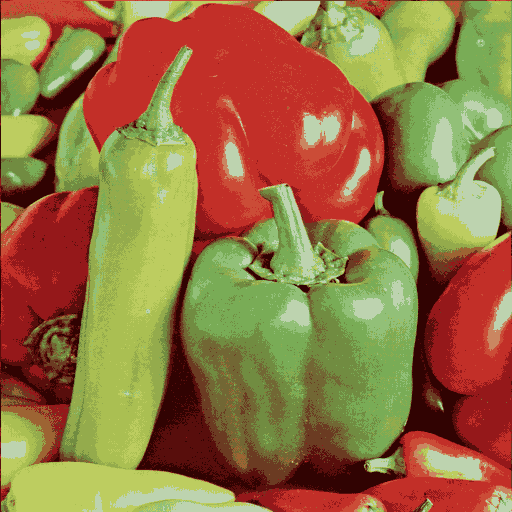
\includegraphics[scale=0.5]{tex/05-k_means/peppers-compressed.png}
	\caption{Compressed image}
\end{figure}
\end{answer}
